\documentclass[tikz,border=2pt]{standalone}
\usepackage{ctex}
\begin{document}
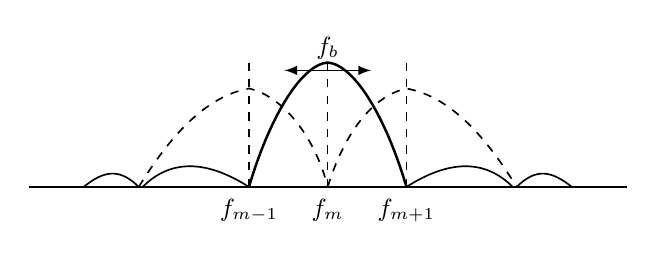
\begin{tikzpicture}[>=latex, font=\small, x=1cm, y=1cm]
\draw[line width=0.6pt] (-3.8,0) -- (3.8,0);

\draw[dashed, line width=0.6pt] (-2.4,0) .. controls (-2.0,0.65) and (-1.55,1.15) .. (-1.0,1.25)
  .. controls (-0.55,1.15) and (-0.15,0.60) .. (0,0);
\draw[dashed, line width=0.6pt] (0,0) .. controls (0.20,0.65) and (0.55,1.15) .. (1.0,1.25)
  .. controls (1.55,1.15) and (2.0,0.65) .. (2.4,0);

\draw[line width=0.9pt] (-1,0) .. controls (-0.75,0.85) and (-0.35,1.55) .. (0,1.58)
  .. controls (0.35,1.55) and (0.75,0.85) .. (1,0);

\draw[line width=0.6pt] (-3.1,0) .. controls (-2.85,0.20) and (-2.65,0.25) .. (-2.4,0);
\draw[line width=0.6pt] (-2.35,0) .. controls (-2.0,0.35) and (-1.55,0.35) .. (-1.0,0);
\draw[line width=0.6pt] (1.0,0) .. controls (1.55,0.35) and (2.0,0.35) .. (2.35,0);
\draw[line width=0.6pt] (2.4,0) .. controls (2.65,0.25) and (2.85,0.20) .. (3.1,0);

\draw[dashed, line width=0.5pt] (-1,0) -- (-1,1.58);
\draw[dashed, line width=0.5pt] (0,0) -- (0,1.58);
\draw[dashed, line width=0.5pt] (1,0) -- (1,1.58);

\draw[<->, line width=0.6pt] (-0.55,1.48) -- (0.55,1.48);
\node[above] at (0,1.50) {$f_b$};

\node[below] at (-1,-0.03) {$f_{m-1}$};
\node[below] at (0,-0.03) {$f_m$};
\node[below] at (1,-0.03) {$f_{m+1}$};
\end{tikzpicture}
\end{document}
